\documentclass{beamer}
\usepackage[utf8]{inputenc}
\usepackage{amsmath}
\usepackage{amssymb}
\usepackage{svg}
\usepackage{cite}

\usetheme{Madrid}
\usecolortheme{default}

%------------------------------------------------------------
%This block of code defines the information to appear in the
%Title page
\title[AE SPDnet]
{Learning distributions on Riemannian manifolds}

\subtitle{Autoencoder for SPD matrices}

\author[CB]
{Charlotte BOUCHERIE, Florian YGER, Thibault DE SURREL}

\institute{LITIS}

\date[2025]
{2025}

%\logo{\includegraphics[height=1cm]{overleaf-logo}}

\AtBeginSection[]
{
  \begin{frame}
    \frametitle{Table of contents}
    \tableofcontents[currentsection]
  \end{frame}
}

%------------------------------------------------------------
% Start of document -- Autoencoder for SPD matrices
%------------------------------------------------------------
\begin{document}

\frame{\titlepage}

\begin{frame}
\frametitle{Table of contents}
\tableofcontents
\end{frame}

%---------------------------------------------------------
\section{Context}
%---
\subsection{Works on SPD matrices}
%---
\begin{frame}
\frametitle{A Riemannian Network for SPD Matrix Learning: SPDnet}
Introduction of a network architecture that preserves the properties of positive definite matrices for Deep Learning \cite{DBLP:journals/corr/HuangG16}
\begin{itemize}
    \item 3 different layers: BiMap, ReEig, LogEig
    \item We will base ourselves on these layers for our autoencoder    
\end{itemize}

\end{frame}
%-
\begin{frame}
    \frametitle{Different works}
    DreamNet: A Deep Riemannian Manifold Network for SPD Matrix Learning \cite{wang2022dreamnetdeepriemanniannetwork}
    \begin{itemize}
        \item Methodology for creating deep networks
        \item Stacked Riemannian Autoencoder (SRAE) at the end of the network
    \end{itemize}
    Riemannian Multinomial Logistics Regression for SPD Neural Networks \cite{chen2024riemannianmultinomiallogisticsregression}
    \begin{itemize}
        \item Adapting logistic regression for SPD matrices
        \item New specific layer for classification
        \item Use of Log-Euclidean Metric or Log-Cholesky Metric
    \end{itemize}
    SPD domain-specific batch normalization to crack interpretable unsupervised domain adaptation in EEG \cite{kobler2022spddomainspecificbatchnormalization}
    \begin{itemize}
        \item Specific batch normalization for SPD matrices
    \end{itemize}
\end{frame}
%-
\begin{frame}
    \frametitle{Different works}
    Riemannian batch normalization for SPD neural networks \cite{brooks2019riemannianbatchnormalizationspd}
    \begin{itemize}
        \item Specific batch normalization for SPD matrices
    \end{itemize}
    A Riemannian Residual Learning Mechanism for SPD Network \cite{10651149}
    \begin{itemize}
        \item Improves learning process for SPD networks
    \end{itemize}
    \frametitle{Different works}
    U-SPDNet: An SPD manifold learning-based neural network for visual classification \cite{WANG2023382}
    \begin{itemize}
        \item SPD matrices from visual data
    \end{itemize}
\end{frame}
%-
\begin{frame}
    \frametitle{Different works}
    Reducing the Dimensionality of SPD Matrices with Neural Networks in BCI \cite{articledimension}
    \begin{itemize}
        \item Simplification of complex data for a better interpretability and processing in BCI data
    \end{itemize}
    Schur's Positive Definite Network: Deep Learning in the SPD Cone With Structure \cite{pouliquen:hal-04726325}
    \begin{itemize}
        \item Shows that the use of the structure in the network improves the performances
    \end{itemize}
    Modeling Graphs Beyond Hyperbolic: Graph Neural Networks in Symmetric Positive Definite Matrices \cite{zhao2023modelinggraphshyperbolicgraph}
    \begin{itemize}
        \item Applies GNN to SPD matrices
        \item To model graph structures in SPD matrices
    \end{itemize}
\end{frame}
%-
\begin{frame}
    \frametitle{Different works}
    SymNet: A Simple Symmetric Positive Definite Manifold Deep Learning Method for Image Set Classification \cite{9390301}
    \begin{itemize}
        \item Image set classification
    \end{itemize}
    From Manifold to Manifold: Geometry-Aware Dimensionality Reduction for SPD Matrices \cite{harandi2014manifoldmanifoldgeometryawaredimensionality}
    \begin{itemize}
        \item Lower-dimensional and more discriminative SPD matrices from SPD matrices with orthonormal projection
    \end{itemize}
    Geometry-Aware Principal Component Analysis for Symmetric Positive Definite Matrices \cite{articlepcaaspd}
    \begin{itemize}
        \item PCA applied to SPD matrices
        \item Preserves more data variance
        \item Extends PCA from Euclidean to Riemannian geometries
    \end{itemize}
\end{frame}
%---
\subsection{Riemannian geometry}
%---
\begin{frame}
    \frametitle{Riemannian geometry}
    Riemann metric \textit{(AIRM)}: $\delta^2_R(X,Y)$ = $||\text{log}(X^{-1/2}YX^{-1/2})||^2_F$
    \begin{itemize}
        \item Measure the similarity between two SPD matrices while respecting the structure
        \item We will use it in our AE in the model, in the cost function and in the trustworthiness.
    \end{itemize}
    Representing information with SPD matrices has proven beneficial for many recognition tasks. 
    Considering Riemannian geometry comes at a high cost especially in high-dimensional ones that limits applicability.
\end{frame}
%-
%---
\subsection{Objectives}
%-
\begin{frame}
\frametitle{Objectives}
How to preserve the SPD matrix through the reconstitutions ?
\begin{itemize}
    \item Autoencoder for SPD matrices for dimension reduction
    \item Layer to do the reverse operations of the autoencoder
    \item Impact of Riamannian or Euclidean distance for reconstruction error
\end{itemize}
\end{frame}
%---------------------------------------------------------
\section{Autoencoder}
\begin{frame}
    \frametitle{Autoencoder Basics}
    \begin{itemize}
        \item Unsupervised learning: measurement of reconstruction error
        \item Dimension reduction
        \item Learn the underlying patterns
        \item Used for generative models
\end{itemize}
\begin{center}
    $ \phi : \mathcal{X} \rightarrow \mathcal{F}$ , encoder \\
    $ \psi : \mathcal{F} \rightarrow \mathcal{X}$ , decoder \\
    $ \phi,\psi = \arg \min\limits_{\phi,\psi} || X-(\psi \circ \phi)(X)||^2$
\end{center}
\begin{center}
    \includesvg[width=0.6\textwidth]{figures/autoencoder.svg}
\end{center}

\end{frame}

%---
\subsection{Metrics}
%--
\begin{frame}
    \frametitle{Reconstruction error}
    \begin{itemize}
        \item For each matrix, we calculate the Riemannian distance with its reconstruction.
    \end{itemize}
    \begin{center}
        $ \phi : \mathcal{X} \rightarrow \mathcal{F}$ \\
        $ \psi : \mathcal{F} \rightarrow \mathcal{X}$ \\
        $ X \in \mathcal{X}$ is SPD \\
        $ \psi (\phi(X)) \in \mathcal{X}$ is SPD \\
        $ \phi,\psi = \arg\min\limits_{\phi,\psi} \delta^2_R(X,\psi (\phi(X))) =  \arg \min\limits_{\phi,\psi} ||\text{log}(X^{-1/2}\psi (\phi(X))X^{-1/2})||^2_F$
    \end{center}
    \end{frame}
    %-
\begin{frame}
\frametitle{Trustworthiness}
\begin{itemize}
    \item For each matrix, we take its k closest matrices in the output space and its closest matrices in the input space.
    \item The distance is the same used to calculate our cost function.
    \item We penalize proportionally to the difference in ranks in the input space.
    \item We do not penalize matrices coming closer together.
\end{itemize}
\begin{center}
    $ T(k) = 1 - \frac{2}{nk(2n-3k-1)} \sum\limits_{i=1}^n\sum\limits_{j\in\mathcal{N}_i^k} \max(0,(r(i,j)-k)) $
\end{center}
\end{frame}
%-
\begin{frame}
\frametitle{Accuracy}
\begin{itemize}
    \item We use MDM (Minimum Distance to Mean) to know the accuracy before reconstituting our matrices.
    \item For each class, a centroid is estimated according to our distance.
    \item We compare the accuracy of original matrices and the accuracy of the reconstructions.
\end{itemize}
\end{frame}
%---
\subsection{Layers}
%--

\begin{frame}
\frametitle{BiMap layer}
\begin{itemize}
    \item The function of this layer is to generate more compact and more discriminative SPD matrices.
    \item Layer which performs a bilinear map $f_b$ to transform the initial matrices into new matrices of lower dimension.
\end{itemize}

\begin{center}
    $ X_k = f_b^{(k)}(X_{k-1};W_k)=W_kX_{k-1}W_k^T$
\end{center}

$W_k$ is of full rank to guarantee that $X_k$ remains SPD.

\begin{block}{Network parameters}
    Number of input filters/channels \textit{hi}, number of output filters/channels \textit{ho}, size of input matrix \textit{ni}, size of output matrix \textit{no}
\end{block}


\end{frame}
%--
\begin{frame}
\frametitle{ReEig layer}
\begin{itemize}
    \item The function of this layer is to improve discriminative performance by introducing nonlinearity, in the same way as ReLU.
    \item Introduction of a non-linear function $f_r$ which corrects the matrices by setting a threshold for low eigenvalues.
\end{itemize}

\begin{center}
    $ X_k = f_r^{(k)}(X_{k-1})=U_{k-1}\max(\epsilon I, \Sigma_{k-1})U_{k-1}^T$
\end{center}

\end{frame}

%--
\begin{frame}
\frametitle{LogEig/ExpEig layers}

\begin{block}{LogEig}
    The function of this layer is to be able to apply Riemann geometry to the output matrix.
\end{block}

\begin{center}
    $ X_k = f_l^{(k)}(X_{k-1})=\log (X_{k-1})=U_{k-1}\log(\Sigma_{k-1})U_{k-1}^T$
\end{center}

\begin{block}{ExpEig}
    The function of this layer is to apply the inverse function of the LogEig layer.
\end{block}

\begin{center}
    $ X_k = f_e^{(k)}(X_{k-1})=\exp (X_{k-1})$
\end{center}

\end{frame}
%---
\subsection{Models}
%--
\begin{frame}
\frametitle{One layer}
\begin{itemize}
    \item Single BiMap layer for the encoder from $ni\rightarrow no$ and $hi\rightarrow ho$.
    \item We look at the influence of the output dimension and the output layer.
    \item The decoder does the opposite operation.
\end{itemize}
\begin{figure}
    \centering
    {\tiny
    \includesvg[width=0.9\textwidth]{figures/one_layer.svg}
    \caption{Model architecture for an autoencoder with one layer}
    }
\end{figure}

\end{frame}

\begin{frame}
\frametitle{Two layers with mirror channels}
\begin{itemize}
    \item Two BiMap layers.
        \begin{itemize}
            \item $ni\rightarrow ni/2$ and $hi\rightarrow ho$.
            \item $ni/2\rightarrow no$ and $ho\rightarrow hi$.
        \end{itemize}
        \item We look at the influence of the number of intermediate channels and the output dimension.
        \item The decoder does the opposite operation.
\end{itemize}
\begin{figure}
    \centering
    {\tiny
    \includesvg[width=\textwidth]{figures/hourglass_channel.svg}
    \caption{Model architecture for an autoencoder with two layers and mirror channels}
    }
\end{figure}

\end{frame}


\begin{frame}
\frametitle{Multiple layers evenly distributed}
\begin{itemize}
    \item Number of BiMap layers set in parameters.
    \item Channels and intermediate matrix sizes based on the number of layers.
    \item The decoder does the opposite operation.
\end{itemize}
\begin{figure}
    \centering
    {\tiny
    \includesvg[width=\textwidth]{figures/regular.svg}
    \caption{Model architecture for an autoencoder with multiple layers evenly distributed}
    }
\end{figure}
\end{frame}

\begin{frame}
\frametitle{Multiple layers halved in dimension}
\begin{itemize}
    \item Number of BiMap layers and filters in layers depends on $ni$ and $no$.
    \item Matrix size divided by two, number of filters multiplied by two at each layer.
    \item The decoder does the opposite operation.
\end{itemize}
\begin{figure}
    \centering
    {\tiny
    \includesvg[width=\textwidth]{figures/by_halves.svg}
    }
    \caption{Model architecture for an autoencoder with multiple layers halved in dimension}
\end{figure}

\end{frame}
%---------------------------------------------------------

\section{Results}
%---

%---
\subsection{Synthetic data}
%--
\begin{frame}
\frametitle{Synthetic data}
\begin{itemize}
    \item We generate data along a geodesic
    \item 300 SPD matrices
    \item Matrices dimensions : $8 \times 8$
    \item 1/2 for training, 1/4 for validation, 1/4 for testing
    \item 2 classes : following different geodesics
\end{itemize}
\end{frame}

%--
\begin{frame}
    \frametitle{One layer}
    \begin{figure}
        \centering
        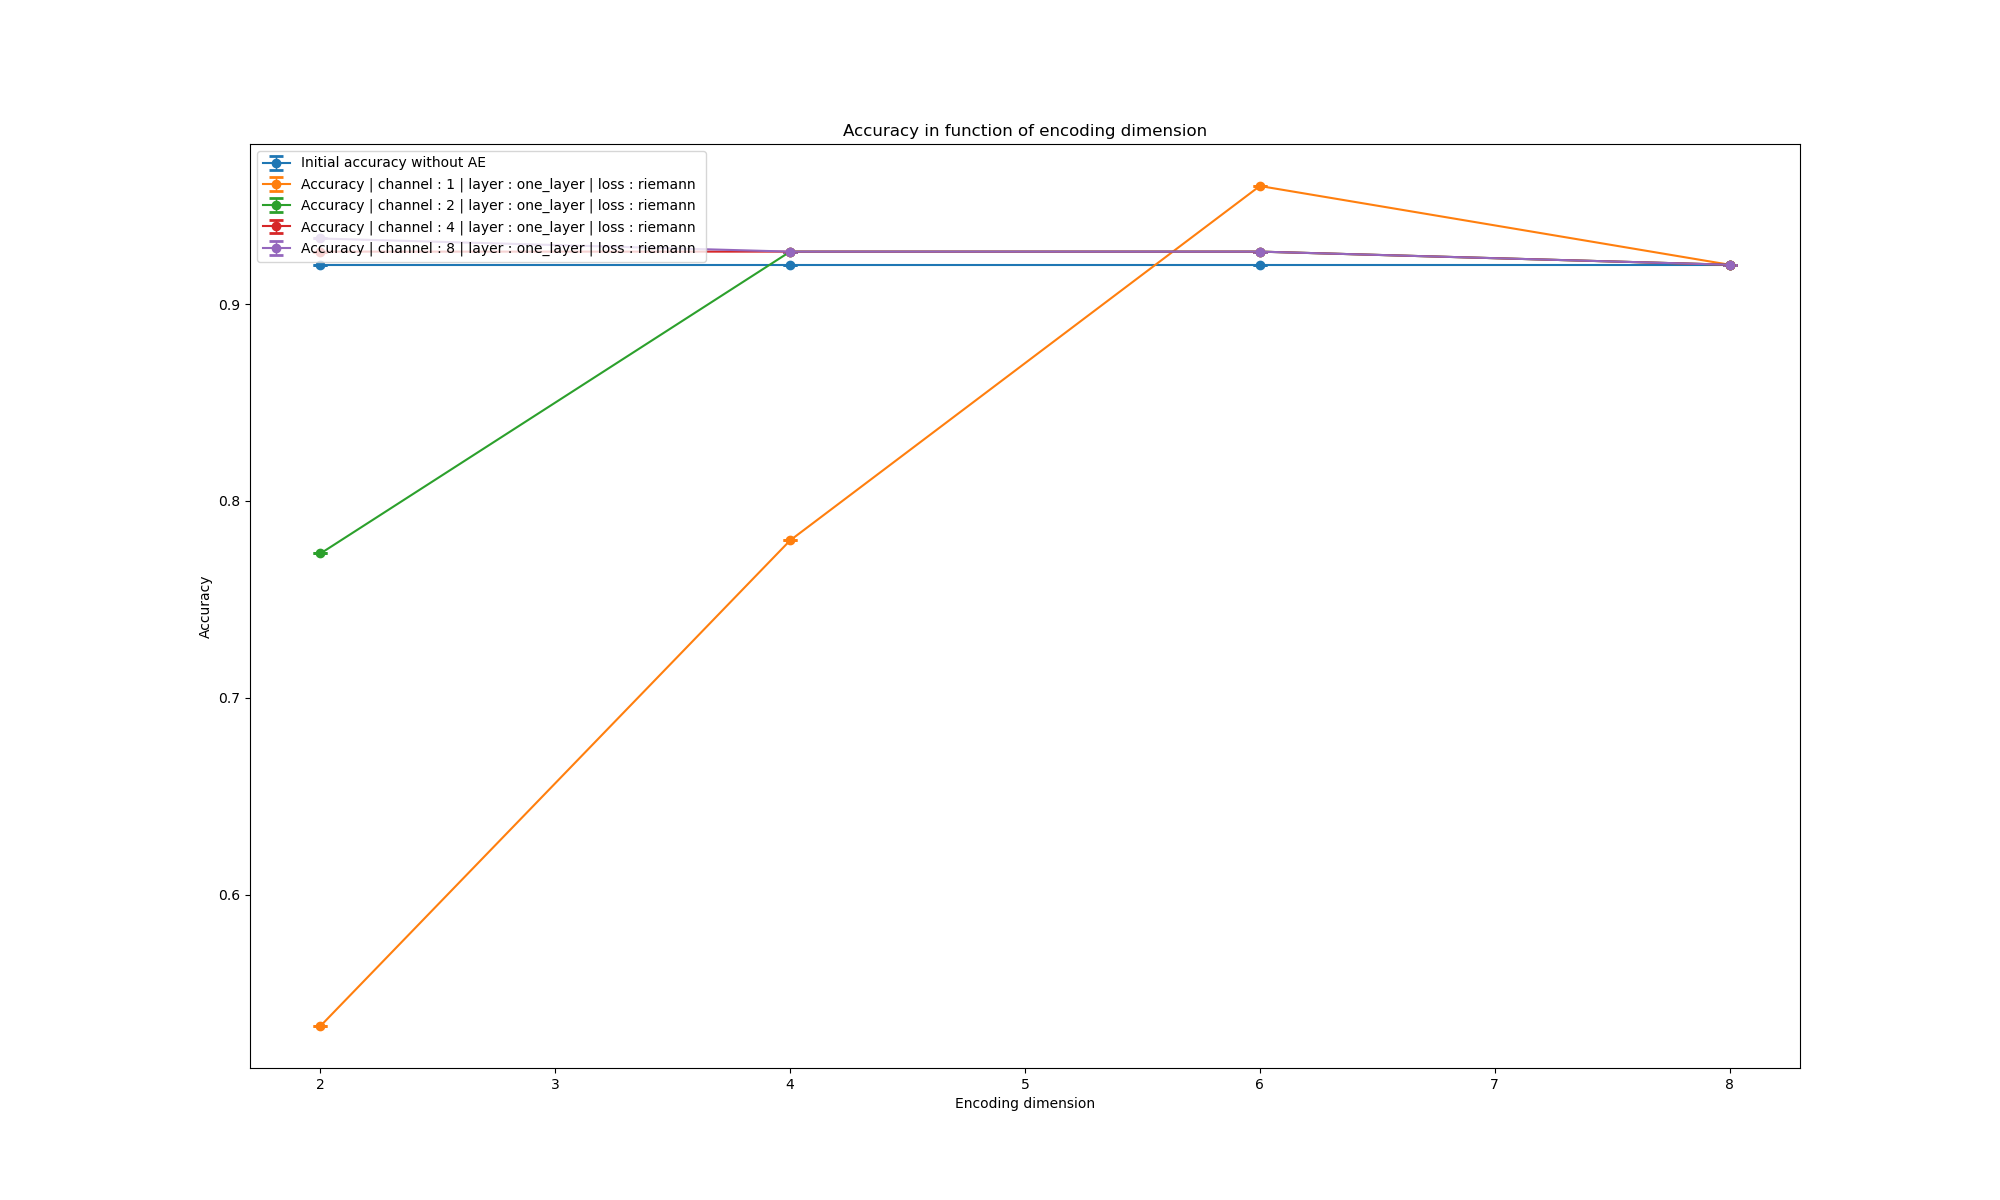
\includegraphics[width=0.4\textwidth]{figures/acc_no_noise_geodesics.png}
        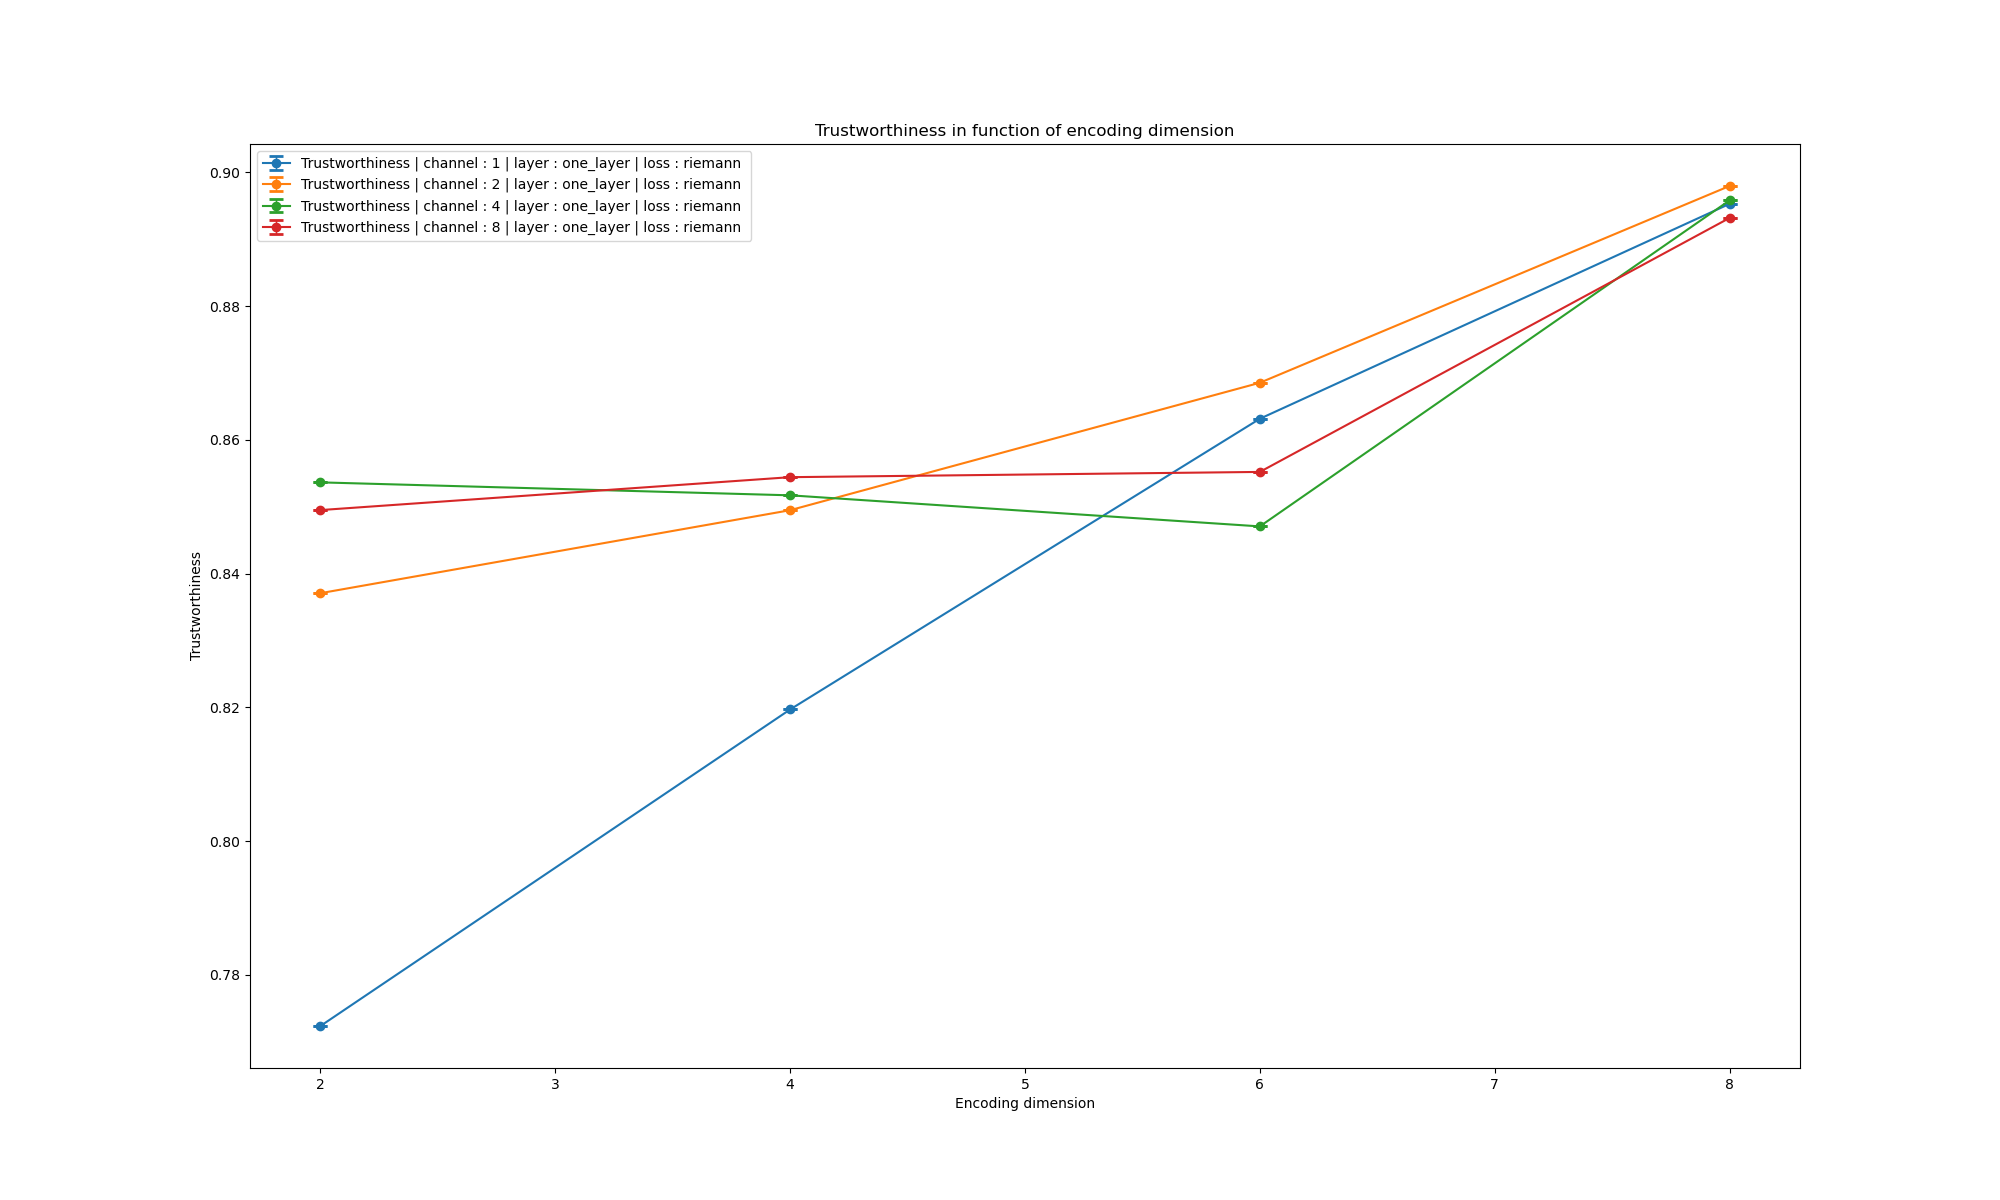
\includegraphics[width=0.4\textwidth]{figures/trustworthiness_geodesics.png}
        \caption{Accuracy and trustworthiness in function of encoding dimensions for different encoding channels with one layer}
    \end{figure}
\end{frame}
%---
\subsection{BCI data}
%---

\begin{frame}
    \frametitle{BCI Data}
    \begin{itemize}
        \item Dataset: BNCI2014\_001
        \item Subject: 8
        \item 144 data samples for training and 144 for testing
        \item 1/3 of the training data used for validation
        \item Covariances matrices dimensions: $22 \times 22$
        \item 2 classes : right hand / left hand
    \end{itemize}
\end{frame}

\begin{frame}
    \frametitle{Multiple layers evenly distributed}
    We fixed the number of layers = 4
    \begin{figure}
        \centering
        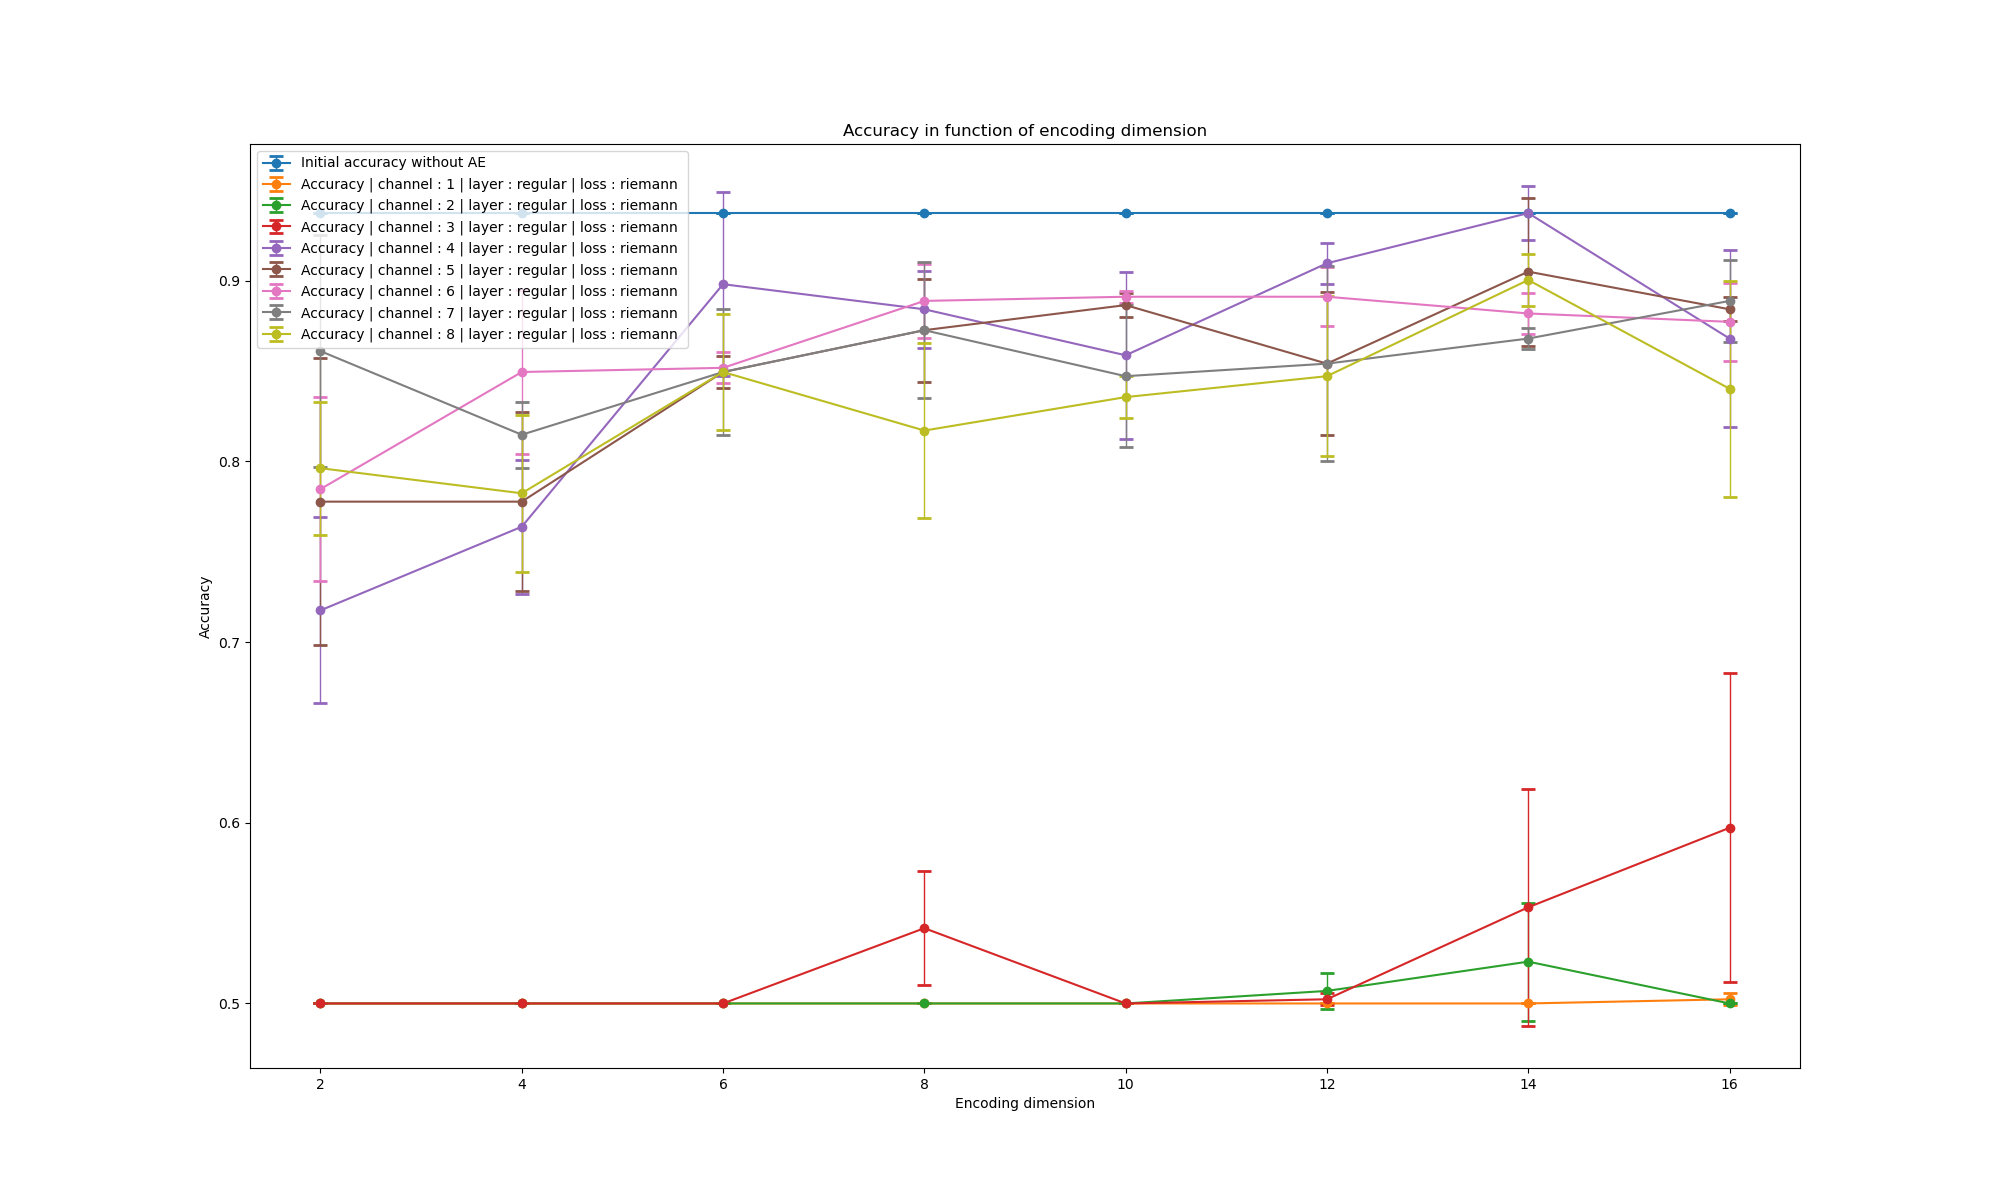
\includegraphics[width=0.8\textwidth]{figures/acc_no_noise_regular_layers.png}
        \caption{Accuracy in function of encoding dimensions for different encoding channels with regular split layers}
    \end{figure}
\end{frame}
    

\begin{frame}
    \frametitle{Denoising autoencoder}
    \begin{center}
        $ \phi : \mathcal{X} \rightarrow \mathcal{F}$ , encoder \\
        $ \psi : \mathcal{F} \rightarrow \mathcal{X}$ , decoder \\
        $ X' = X + noise $ \\
        $ \phi,\psi = \arg \min\limits_{\phi,\psi} || X-(\psi \circ \phi)(X')||^2$ \\
    \end{center}
    \begin{itemize}
        \item We train the model with noised datas
        \item We calculate the reconstruction error between the initial data (before adding noise) and the reconstruction
    \end{itemize}

\end{frame}

\begin{frame}
    \frametitle{Gaussian noise on EEG data}
    \begin{itemize}
        \item We add symmetric Gaussian noise $\epsilon \epsilon^T$ to each of our initial matrices.
        \item We lose accuracy.
    \end{itemize}
    
    \begin{figure}
        \centering
        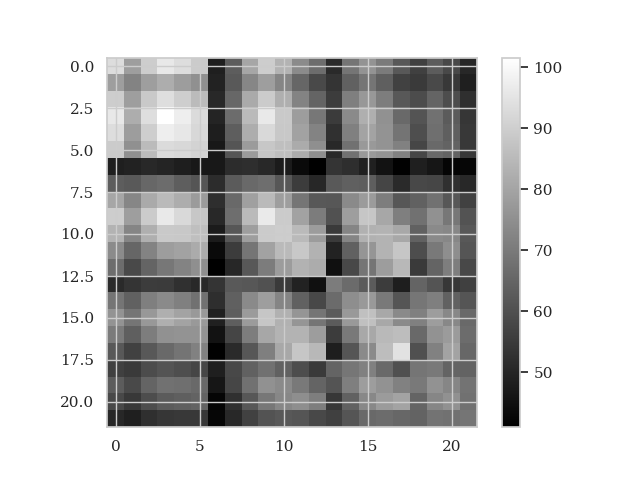
\includegraphics[width=0.3\textwidth]{figures/channel4_encoding_dim10_example_input_test.png}
        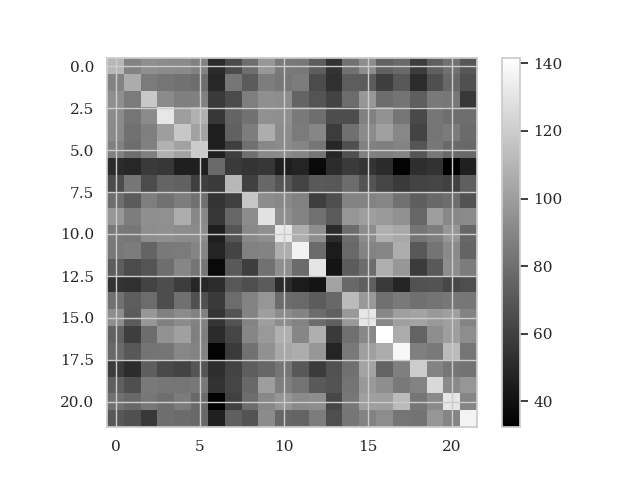
\includegraphics[width=0.3\textwidth]{figures/channel4_encoding_dim10_example_noised_test.png}
        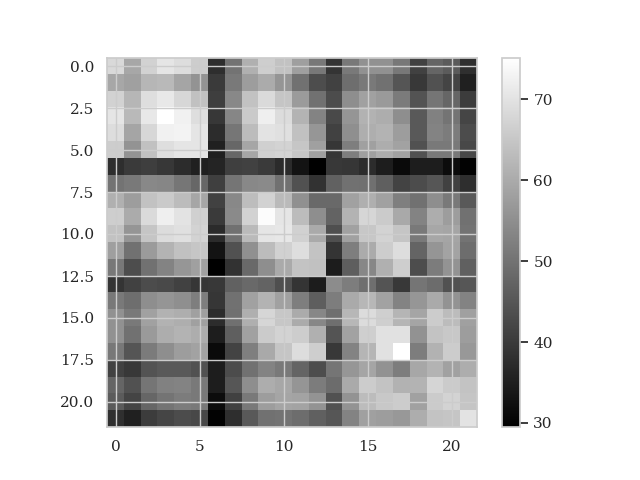
\includegraphics[width=0.3\textwidth]{figures/channel4_encoding_dim10_example_reconstruction_test.png}
        \caption{Effect of Gaussian noise on EEG data: (Left) Original input, (Middle) Noised data, (Right) Reconstruction after noise removal.}
    \end{figure}
\end{frame}

\begin{frame}
    \begin{figure}
        \centering
        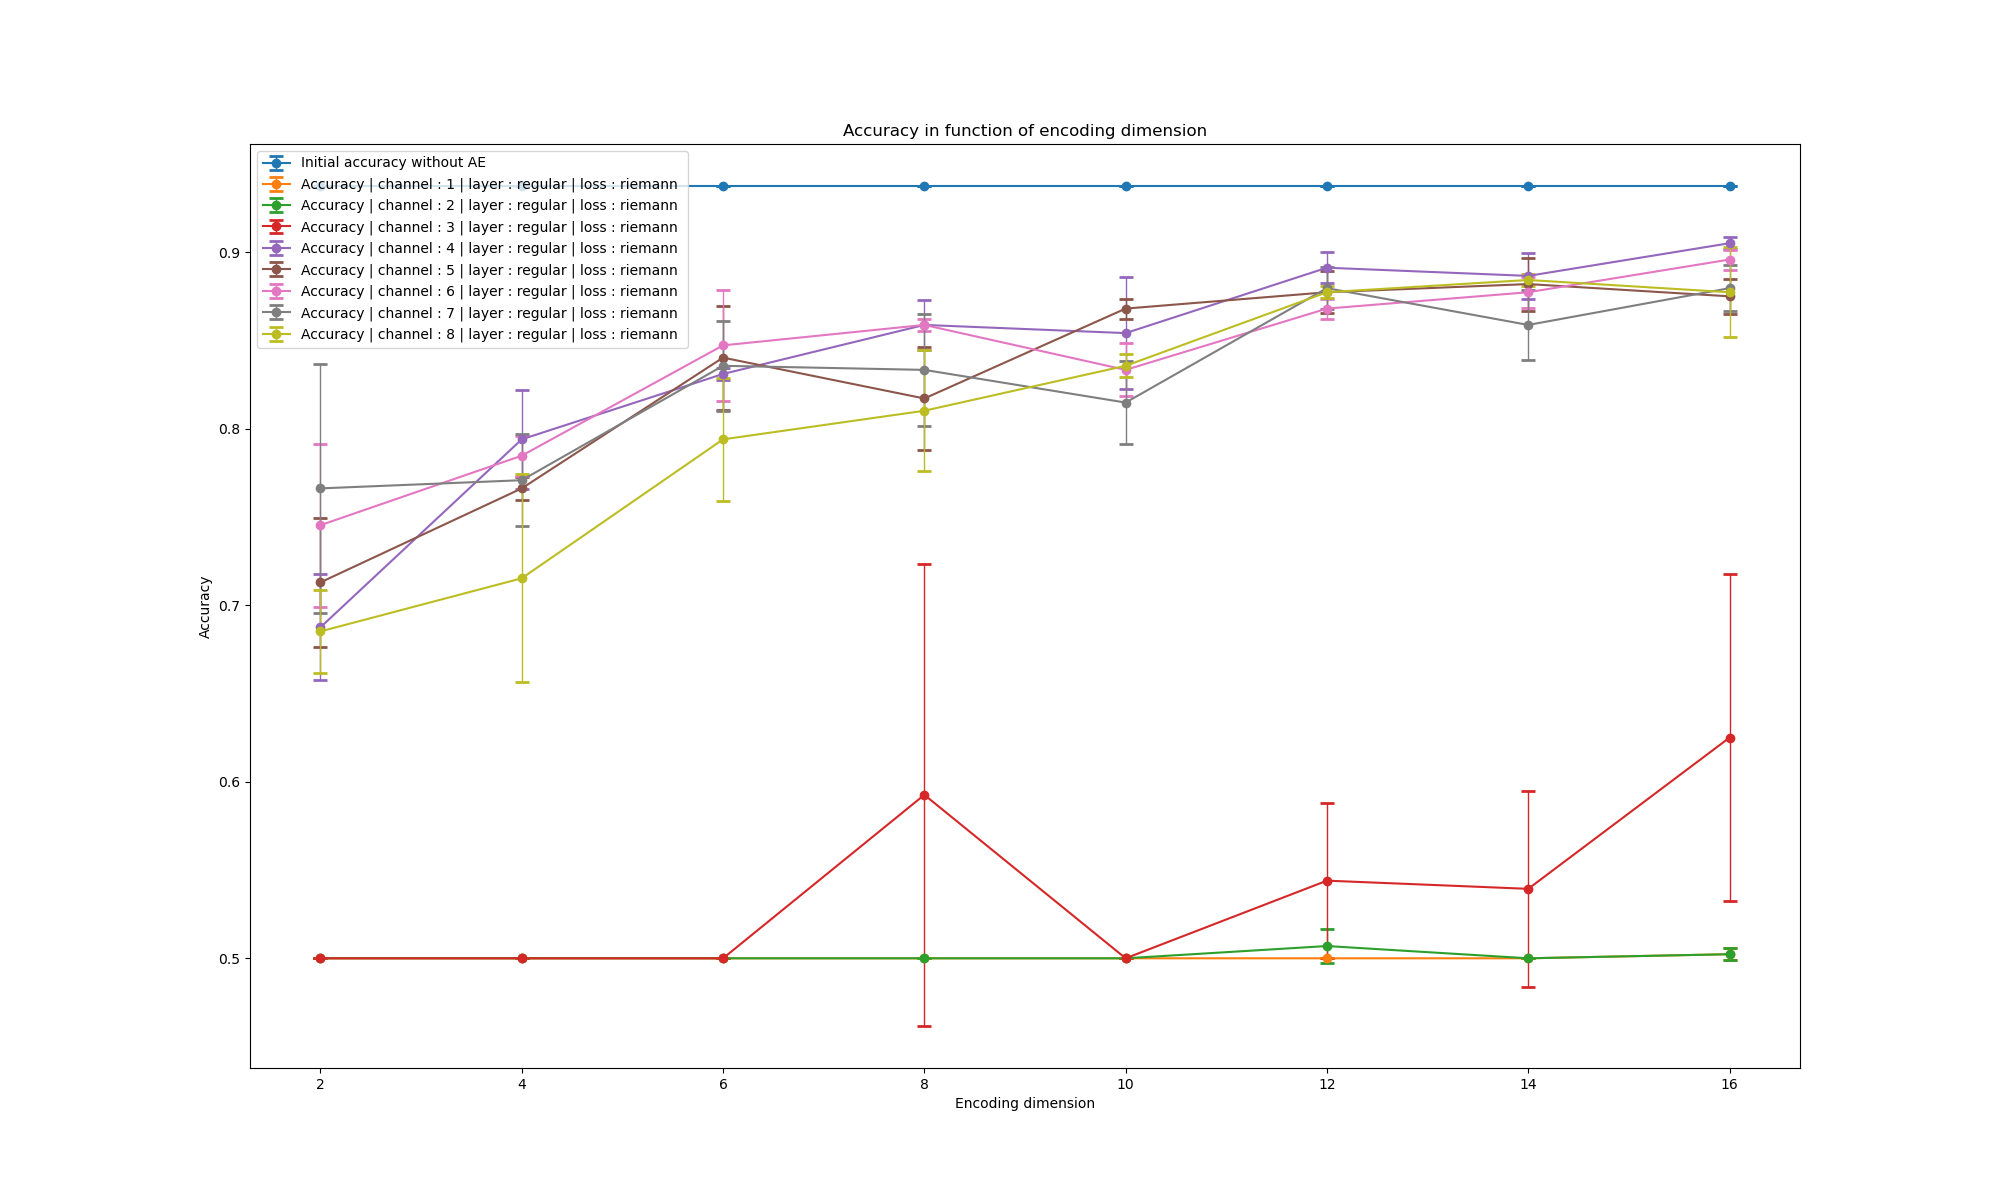
\includegraphics[width=\textwidth]{figures/acc_noise_regular.png}
        \caption{Accuracy in function of encoding dimensions for different encoding channels with noised data with regular split layers}
    \end{figure}
\end{frame}

%-
\begin{frame}
    \frametitle{Ideas}
    \begin{itemize}
        \item Dataset with more complex datas 
        \item Influence of dropout layer/masking noise
    \end{itemize}
\end{frame}

%---------------------------------------------------------
\begin{frame}[allowframebreaks]
    \frametitle{References}
    \bibliographystyle{plain}
    \bibliography{bibtex}
\end{frame}


%---------------------------------------------------------
\end{document}